\documentclass[a4paper,oneside,DIV=12,12pt]{scrartcl}

%%% Color
\usepackage{xcolor}
\definecolor{lightblue}{HTML}{03A9F4}
\definecolor{red}{HTML}{F44336}
%%%

%%% Font settings
\usepackage{fontspec}
\setmainfont{Source Serif Pro}[
	UprightFeatures = {SmallCapsFeatures = {LetterSpace = 5}},
]
\setsansfont{Source Sans Pro}[
]
\setmonofont{Source Code Pro}[
]

\newfontfamily{\titlefont}{Source Serif Pro}[
	FontFace = {xb}{n}{Font = * Black}, % xb for ExtraBold
]

%%% Create weight selection commands for titling font
%% Black
\DeclareRobustCommand{\xbseries}{\fontseries{xb}\selectfont}
\DeclareTextFontCommand{\textxb}{\xbseries}
%%%

\setkomafont{disposition}{\titlefont\bfseries}
\setkomafont{pagenumber}{\rmfamily}

\usepackage{microtype}
%%%


%%% Language specific
\usepackage{polyglossia}
\setmainlanguage{russian}
%%%

%%% Enumerated lists
\usepackage{enumitem}
\newlist{steps}{enumerate}{10}
\setlist[steps]{
	label*=\arabic*.,
	% leftmargin = 0em,
	leftmargin = *,
}
%%%

%%% URL and cross-references
\usepackage{hyperref}
\hypersetup{
	colorlinks      = false,
	linkbordercolor = red,
	urlbordercolor  = lightblue,
	pdfborderstyle  = {/S/U/W 1.5},
}
%%%

%%% Graphics inclusion
\usepackage{graphicx}
%%%

%%% User command definitions
\newcommand{\MyDocTitle}[1]{{\centering\titlefont\xbseries\Large#1\par}\vspace{3\baselineskip}} % \normalsize used to get the body text leading
\newcommand{\progname}[1]{\texttt{#1}}

\newcommand{\allcaps}[1]{%
	{\addfontfeatures{LetterSpace = 5}#1}%
}
\newcommand{\emphsc}[1]{\textsc{#1}}
\newcommand{\Attention}[1]{\noindent\textsc{Внимание!}~#1\par}
%%%

\begin{document}
	\MyDocTitle{Из C или C++ в язык ассемблера}
	
	% \tableofcontents
	
	\section{Что это?}
		Эта инструкция описывает, как получать код на языке ассемблера из исходного кода, написанного на языках C или C++, а также как его собирать в рабочую программу.
		
	\section{Перед работой}
		Чтобы превратить код рабочей программы на C или C++ понадобится только совместимый компилятор: \progname{clang} или \progname{gcc}. Для Windows удобнее устанавливать \progname{gcc} — он входит в комплект поставки всего одной программы.
		
		Для установки \progname{gcc} на Windows достаточно скачать и установить пакет \allcaps{MSYS2} (\url{https://www.msys2.org/}) и собственно сам \progname{gcc}. На других операционных системах, вроде Linux, BSD и macOS, любой из компиляторов легко устанавливается с помощью пакетного менеджера (\progname{apt}, \progname{brew}, \progname{pacman} и так далее), а \progname{gcc} есть ещё с момента установки ОС.
		
	\section{Как пользоваться?}
		Процесс состоит из нескольких шагов: настройка среды, разработка программы, получение кода на языке ассемблера и сборка ассемблерного кода.
		
		\subsection{Настройка среды}
			Настройка среды выполняется \emphsc{только первый раз} и нужна исключительно для полной установки \allcaps{MSYS2} и компилятора.
			\begin{steps}[ref={\arabic*}]
				\item \label{installpath} Установить и обновить \allcaps{MSYS2}, следуя инструкциям на сайте. Устанавливайте версию, которая соответствует разрядности вашей операционной системы: 32-битную версию для 32-битной ОС, 64-битную для 64-битной. Обратите внимание на путь, куда устанавливается программа. По умолчанию для 32-бит\-ной версии это «\path{C:\msys32\}», для 64-битной~— «\path{C:\msys64\}». Запомните этот путь! Он понадобится дальше.
				
				\item Открыть оболочку \allcaps{MSYS2} MinGW, запустив программу «\allcaps{MSYS2} MinGW 32-bit» на 32-битной системе или «\allcaps{MSYS2} MinGW 64-bit» на 64-битной.
				
				\item Установить \progname{gcc} с помощью такой команды:
				\begin{verbatim}
pacman -S $MINGW_PACKAGE_PREFIX-gcc
				\end{verbatim}
				
				\item Закрыть оболочку \allcaps{MSYS2} с помощью команды:
				\begin{verbatim}
exit
				\end{verbatim}
				
				\item Добавить папку исполняемых файлов в переменную \texttt{PATH}. Для этого зайти в «Панель управления» → «Система» → «Дополнительные параметры системы» (в боковом меню) → «Переменные среды…» (кнопка снизу). В части окна, подписанной «Переменные среды пользователя для…» найти переменную \texttt{path} (регистр не важен: \texttt{Path}, \texttt{PATH}~— одинаковые имена). В поле «Значение переменной» дописать путь, который вы запомнили в шаге~\ref{installpath}, добавив в него строку «\path{\mingw(32 или 64)\bin}». Если в поле уже есть какое-то значение, \emphsc{не удаляйте его!}
				
				Например, если у вас 32-битная операционная система и \allcaps{MSYS2} установлен в папку~«\path{C:\msys32\}», то в поле нужно дописать «\path{C:\msys32\mingw32\bin}». Если же система 64-битная и \allcaps{MSYS2} установлен в папку~«\path{C:\msys64\}», то в поле нужно дописать «\path{C:\msys64\mingw64\bin}». Если поле не пустое, то есть уже содержит какие-то другие пути, перед строкой, которую вы вставляете, введите символ «;». Пример на рис.~\ref{fig:append-to-path}.
				
				\item Убедиться, что все команды выполнены правильно. Для этого открыть командную строку Windows (\progname{cmd.exe}) и выполнить команду:
				\begin{verbatim}
gcc --version
				\end{verbatim}
				Среда настроена и готова к работе, если вывод вышеописанной команды выглядит примерно так:
				
				{\ttfamily
gcc (Rev1, Built by MSYS2 project) 7.3.0\\
Copyright (C) 2017 Free Software Foundation, Inc.\\
This is free software; see the source for copying conditions.  There is NO
warranty; not even for MERCHANTABILITY or FITNESS FOR A PARTICULAR PURPOSE.}
			\end{steps}
			
			\begin{figure}[!htbp]
			\centering
				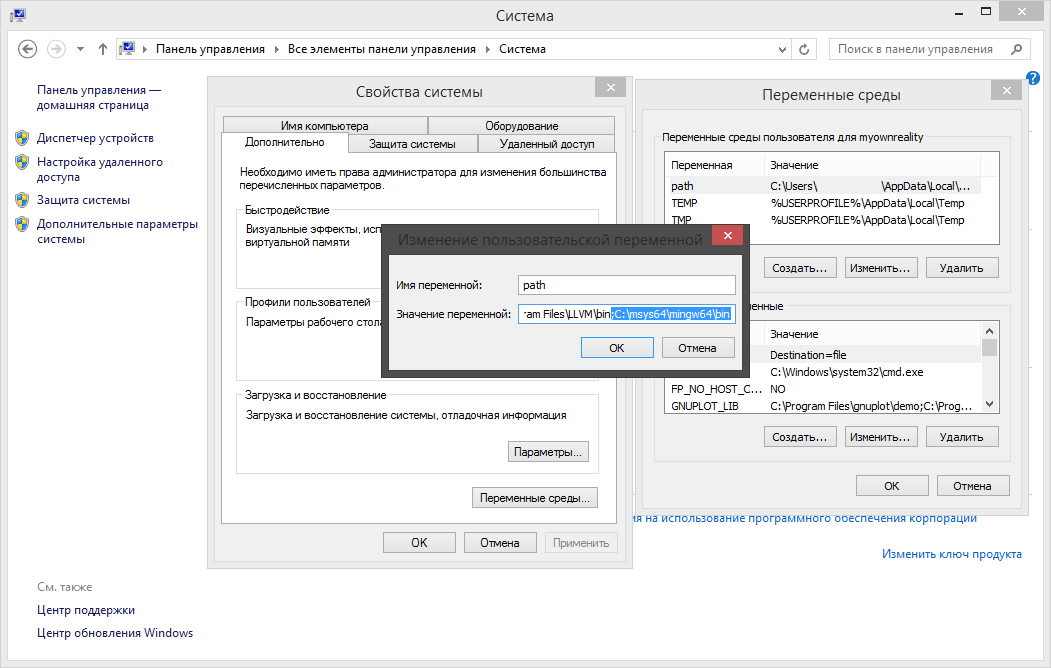
\includegraphics[width = \textwidth]{assets/append-to-path.png}
			\caption{Добавление папки с исполняемыми файлами в переменную \texttt{PATH}}
			\label{fig:append-to-path}
			\end{figure}
		
		\subsection{Разработка программы}
			Раздел для тех, кто всю жизнь пользовался Visual Studio и другими \allcaps{IDE} и не собирал исходники руками.
			\begin{steps}
				\item Написать нужную программу на C или C++, сохранив её текст в файл с соответствующим расширением (\verb|.c| или \verb|.cpp|). Например, \texttt{example.c}.
				\item Открыть командную строку в папке с файлом исходного кода. Если открыто окно Проводника в нужной папке, то удобнее всего это делается с помощью комбинации клавиш «Shift + Правая Клавиша Мыши» — «Открыть окно команд».
				\item Скомпилировать нужную программу. Например, для программы с исходным кодом в файле \texttt{example.c}\footnote{Если программа написана на C++, то тут и далее нужно заменить \texttt{gcc} на \texttt{g++}, а расширение файла с \texttt{.c} на~\texttt{.cpp}.}:
					\begin{verbatim}
gcc example.c
					\end{verbatim}
				% Если исходный код написан на языке C++ и находится в файле \verb|example.cpp|, то компилировать нужно так:
					% \begin{verbatim}
% g++ example.cpp
					% \end{verbatim}
				В результате будет создан исполняемый файл \verb|a.exe|.
				\item Убедиться, что программа работает как нужно, запустив программу из командной строки:
				\begin{verbatim}
a.exe
				\end{verbatim}
			\end{steps}
			Важно убедиться, что программа работает правильно, чтобы собирать ассемблерный код только один раз. 
		
		\subsection{Получение кода на языке ассемблера}
			Если программа работает правильно, можно приступать к получению кода на языке ассемблера. Для этого нужно:
			\begin{steps}
				\item Запустить сборку программы со специальными параметрами. На примерe \verb|example.c|:
				\begin{verbatim}
gcc -S -masm=intel example.c
				\end{verbatim}
			\end{steps}
			В результате будет создан файл \verb|example.s|, который и содержит код на языке Ассемблера. Название зависит от названия файла с вашим исходным кодом на C или C++, но файл с кодом на языке ассемблера всегда будет иметь расширение~\verb|.s|.
			
			Параметр \verb|-S| говорит компилятору производить код на языке ассемблера. Параметр \verb|-masm| со значением \verb|intel| говорит, что результирующий код должен быть написан на синтаксисе Intel. Именно этот синтаксис используется в тексте лаб, да и вообще используется чаще. Также можно использовать значение \texttt{att}, если нужен код с использованием синтаксиса AT\&T. Этот параметр никак не зависит от производителя процессора.
			
		\subsection{Сборка ассемблерного кода}
			Превращение полученного кода на языке ассемблера в работающую программу выполняется компилятором. «Чистые» ассемблеры (\progname{nasm}, \progname{tasm}, \progname{yasm}) обычно не могут этого сделать. Скорее всего, потому что компилятор оставляет специальные директивы для компоновщика (линкера) и использует некоторые собственные директивы, например, \verb|.seh_stackalloc|. Таким образом, чтобы собрать полученный код, нужно:
			\begin{steps}
				\item Запустить сборку файла исходного кода на языке ассемблера:
				\begin{verbatim}
gcc example.s -o example.exe
				\end{verbatim}
			\end{steps}
			В результате будет создан исполняемый файл \verb|example.exe|. Если вы выполнили все предыдущие этапы (у вас настроена среда и есть исходники рабочей программы), то вам нужен только сгенерированный код (файл~\verb|example.s|). При сдаче лабы стоит выполнять \emphsc{только этот этап.} Остальные файлы из папки можно удалить или переместить.
			
	\section{Visual Studio}
		Для тех, у кого установлен Visual Studio, можно попытаться сделать то же самое с помощью установленных \verb|cl.exe| и \verb|ml.exe|. Если исходный код вашей программы записан в файле \verb|example.c|, то получить код на языке ассемблера можно такой командой:
		\begin{verbatim}
cl.exe /FA example.c
		\end{verbatim}
		В результате должен быть создан файл \verb|example.asm|. Чтобы собрать полученный файл в программу нужно выполнить такую команду:
		\begin{verbatim}
ml.exe /nologo example.asm
		\end{verbatim}
		
		\Attention{Все данные по Visual Studio вслепую взяты из \allcaps{MSDN}. Я не могу проверить работоспособность этих команд, так что их правильную работу я не гарантирую.}
\end{document}